Nas subseções seguintes, são verificados os efeitos dos seguintes choques
(i) aumento na taxa de crescimento do investimento residencial; (ii) aumento na participação dos salários na renda e; (iii) aumento na taxa de juro. Os resultados são comparados com um cenário \textit{baseline} representado pela linha tracejada e são apresentados na tabela \ref{Resumo_Simulacao}.

\section{Simulação e choques}

\subsection{Aumento na taxa de crescimento do investimento residencial}

%Um aumento da taxa de crescimento dos gastos autônomos ($\uparrow g_Z$) causa uma maior taxa de crescimento da demanda que, por sua vez, implica em um maior grau de utilização. Em seguida, de acordo com o princípio do ajuste do estoque de capital, as firmas revisam seus planos de investimento e, consequentemente, altera a propensão marginal a investir de forma que o grau de utilização se ajusta lenta e gradualmente ao desejado. No longo prazo, (i) taxa de crescimento da economia converge a taxa dos gastos autônomos; (ii) como resultado, a propensão marginal a investir é permanentemente mais elevada em relação ao \textit{baseline}; (iii) grau de utilização converge ao normal.

Um aumento da taxa de crescimento dos gastos autônomos ($g_Z$) significa uma maior taxa de crescimento da demanda que inicialmente implica um maior grau de utilização da capacidade produtiva. Em seguida, de acordo com o princípio do ajuste do estoque de capital, as firmas revisam seus planos de investimento e, consequentemente, alteram a propensão marginal a investir de forma que o grau de utilização se ajuste lenta e gradualmente ao desejado. A mudança da propensão marginal a investir faz com que temporariamente a economia cresça mais rápido que os gastos autônomos. Ao fim dos processos de ajustamento: a (i) taxa de crescimento da economia converge a taxa dos gastos autônomos; (ii) a propensão marginal a investir é permanentemente mais elevada em relação ao \textit{baseline}; (iii) grau de utilização converge ao normal.

%Tais resultados, no entanto, são os esperados seguindo a literatura do supermultiplicador sraffiano. A especificidade deste modelo, como destacado, é a existência de dois tipos de estoques de capital uma vez que as famílias também investem. Como resultado do aumento de $g_Z$, há um efeito positivo sobre a taxa de acumulação de modo que a participação do estoque de capital criador de capacidade aumente em relação ao estoque de capital total da economia ($\uparrow k$). 


Tais resultados estão de acordo com a literatura do supermultiplicador sraffiano e explicitados na figura 5 a seguir. A especificidade deste modelo, como destacado, é a existência de dois tipos de estoques de capital uma vez que as famílias também investem. Um resultado que pode parecer contraintuitivo é que uma maior taxa de crescimento do investimento residencial tem como resultado uma redução  da sua participação no estoque de capital total (isto é, um amento de $k$).

% desenvolver essa ideia tanto pela equação 41, como pela lógica economica. O investimento das firmas hiper reage ao maior crescimento. 

\subsection{Aumento da participação dos salários na renda}
%esse parágrafo ficou bem confuso
%O aumento no \textit{wage-share} gera efeitos positivos sobre a taxa de crescimento da economia e também sobre o grau de utilização, conforme mostra a figura 6(a). No entanto, tais efeitos são temporários uma vez que a taxa de crescimento dos gastos autônomos não é alterada. Isso é refletido no aumento do grau de utilização mesmo estando abaixo do desejado em alguns períodos dada a convergência da taxa de crescimento da economia a $g_Z$ de modo que: (i) taxa de crescimento média é maior que a inicial, mas converge para $g_Z$ no longo prazo; (ii) o aumento na propensão marginal a investir é temporário e retorna ao valor do \textit{baseline}; (iii) grau de utilização converge ao normal mais rapidamente em relação ao choque anterior. 

O aumento no \textit{wage-share} gera efeitos positivos sobre a taxa de crescimento da economia e também sobre o grau de utilização, conforme mostra a figura \ref{choque_2}. No entanto, tais efeitos são temporários uma vez que a taxa de crescimento dos gastos autônomos não é alterada.Com isso temos que: (i) o aumento na propensão marginal a investir é temporário e retorna ao valor do \textit{baseline}; (ii) grau de utilização converge ao normal mais rapidamente em relação ao choque anterior. 

Por fim, apesar do efeito sobre a taxa de crescimento ser temporário, tem efeitos persistentes sobre a participação do capital das firmas no estoque total de capital da economia. Tal resultado decorre da maior taxa de acumulação no início do choque uma vez que a taxa de crescimento do investimento residencial é mantida constante. 

\subsection{Aumento da taxa de juros}

Um aumento da taxa de juros não possui efeitos tanto sobre a taxa de crescimento quanto sobre o grau de utilização da economia (figura \ref{choque_3}). Uma vez que não se altera o grau de utilização, a propensão marginal a investir permanece inalterada. Além disso, como não possui efeitos sobre a taxa de acumulação, 
%a relação $Ik$ 
a relação entre os dois estoques de capital permanece constante. O único efeito é o aumento do comprometimento da renda disponível das famílias com o pagamento dos juros hipotecários\footnote{Neste caso, verifica-se tanto um aumento no pagamento de juros dos depósitos quanto uma diminuição da poupança das famílias e, portanto, dos depósitos. Ambos os efeitos contribuem para o aumento do grau de endividamento das famílias.}. Tal efeito, por sua vez, é maior do que o rendimento dos depósitos de modo o endividamento das famílias aumente\footnote{Expresso como:
$$
\frac{r_m\cdot M_{-1} - r_{mo}\cdot MO_{-1}}{YD}
$$
}. Portanto, os demais resultados de longo prazo são preservados.


\begin{figure}[htb]
    \centering
    \label{choque_1}
    \caption{Efeito de um aumento na taxa de crescimento dos gastos autônomos}
    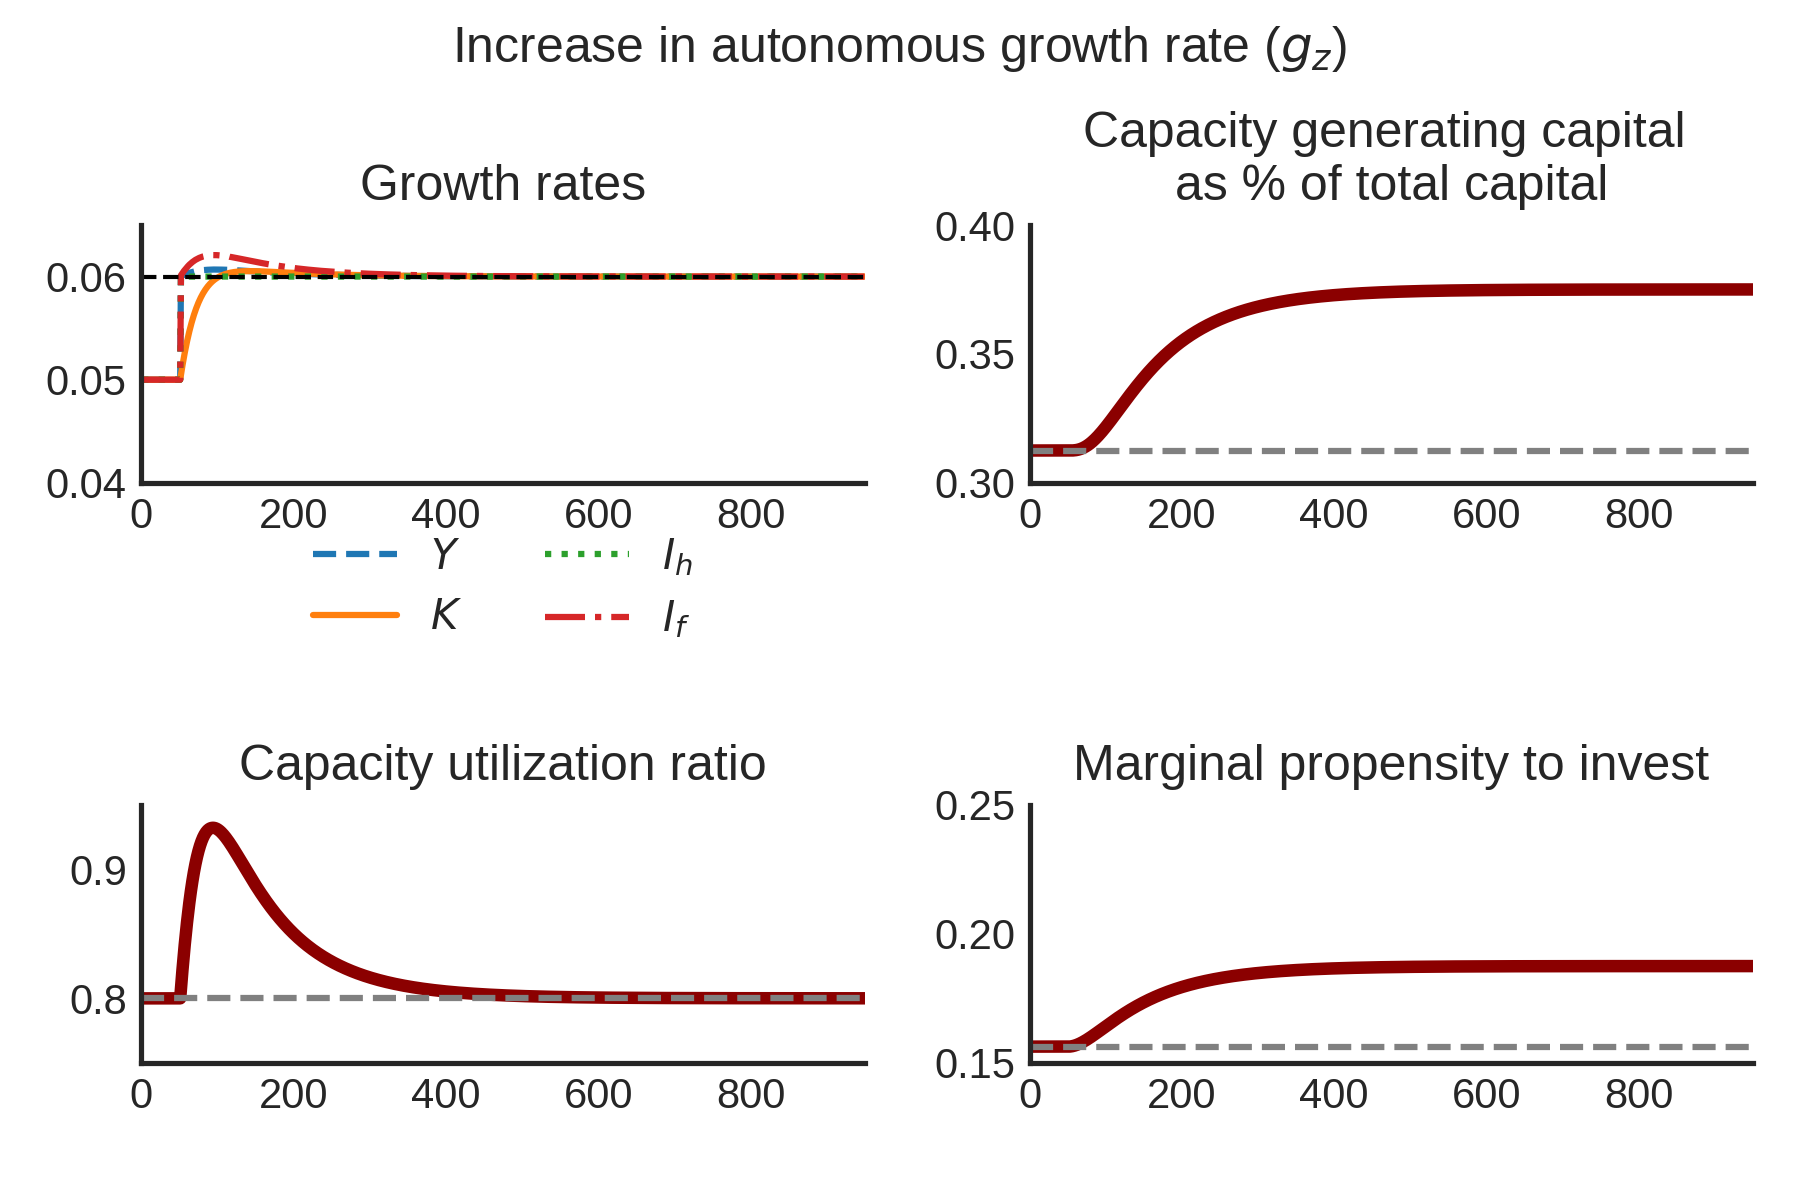
\includegraphics{Modelo/Shock_1.png}
    \caption*{\textbf{Fonte:} Elaboração própria}
\end{figure}


\begin{figure}[htb]
     \centering
     \caption{Resultado dos demais choques}
     \begin{subfigure}[b]{0.45\textwidth}
         \centering
        \caption{Distribuição de renda a favor dos salários}
        \label{choque_2}
        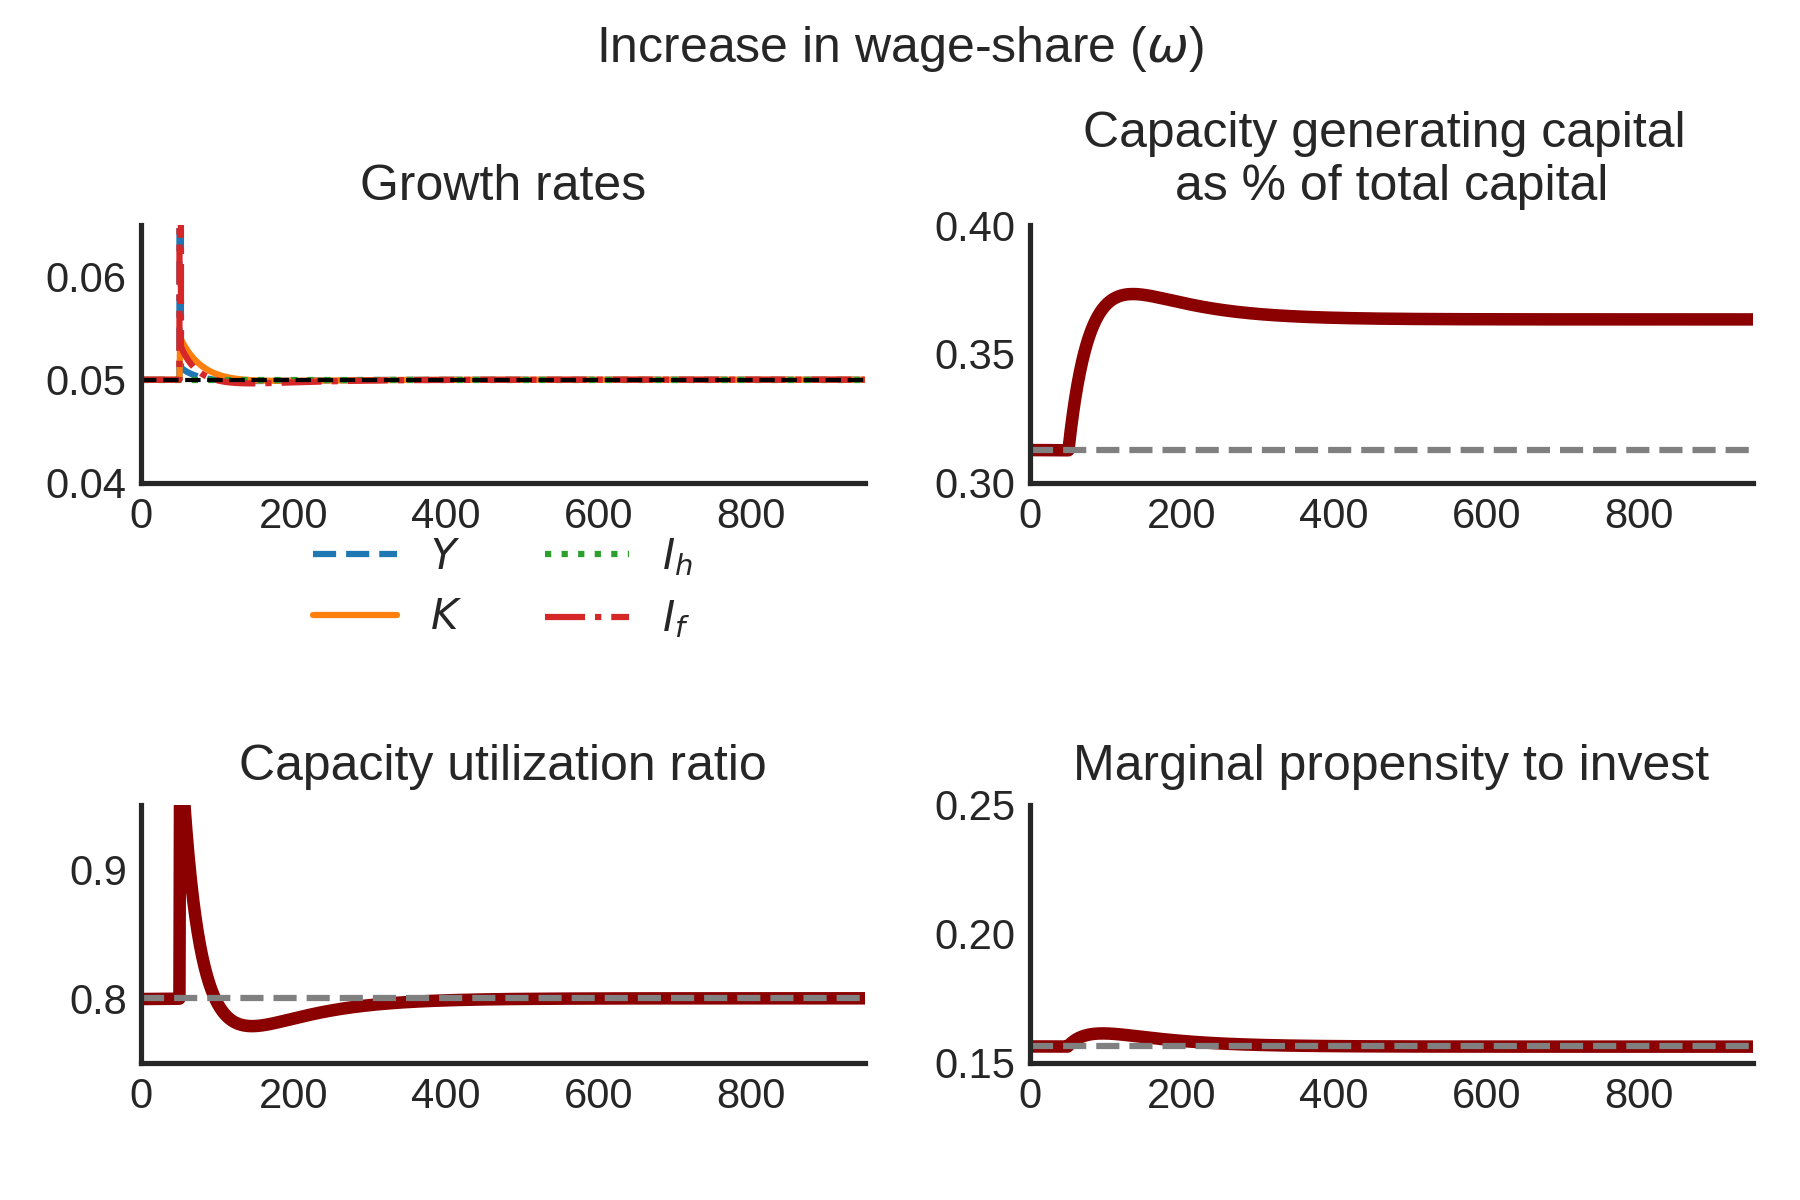
\includegraphics[width = 1\textwidth]{Modelo/Shock_2.png}
     \end{subfigure}
     \hfill
     \begin{subfigure}[b]{0.45\textwidth}
         \centering
         \caption{Aumento na taxa de juros dos depósitos}
         \label{choque_3}
         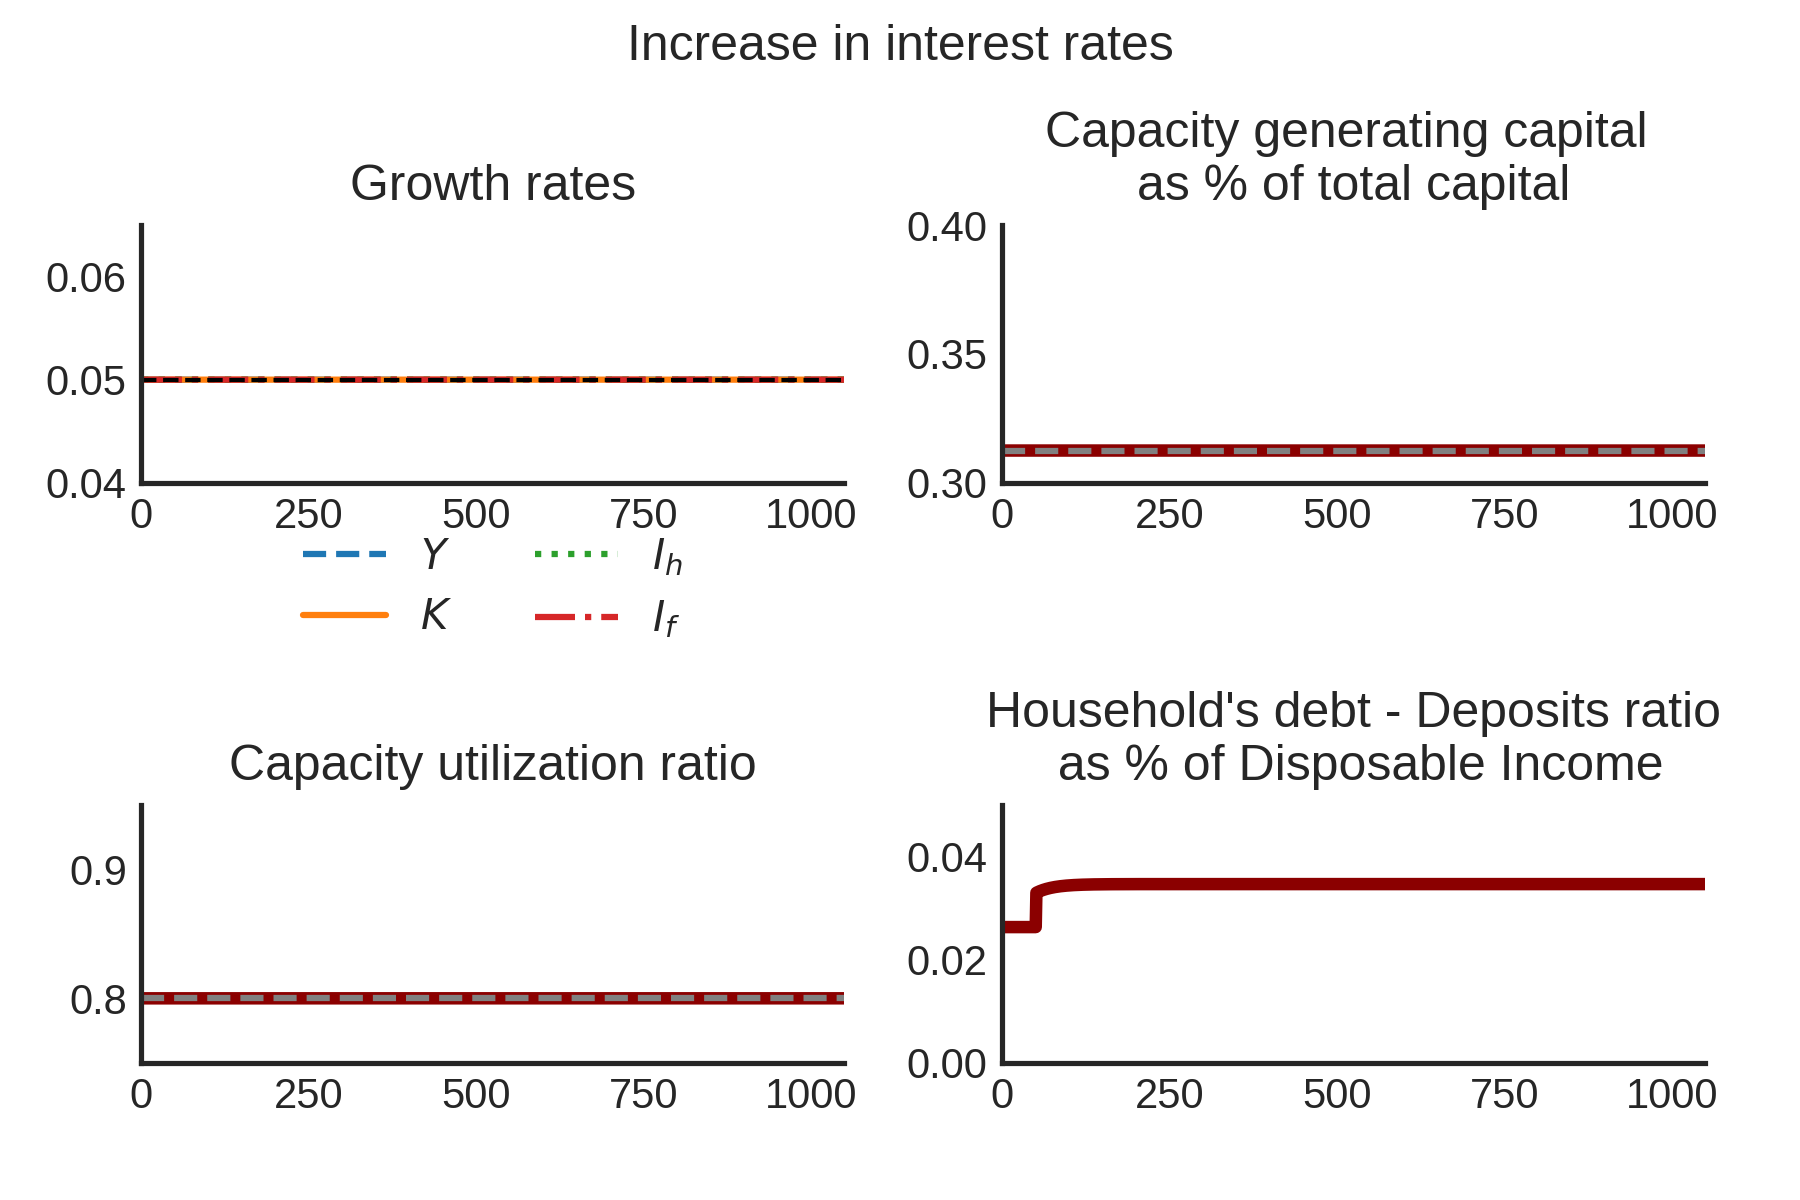
\includegraphics[width = 1\textwidth]{Modelo/Shock_3.png}
     \end{subfigure}
        \caption*{\textbf{Fonte:} Elaboração própria}
        \label{choques}
\end{figure}


\begin{table}[htb]
    \centering
    \caption{Resumo das simulações}
    \label{Resumo_Simulacao}
         \begin{tabular}{ccccc}
\toprule
{} &  Base scenario &  $\Delta g_Z$ &  $\Delta \omega$ &  $\Delta rm$ \\
\midrule
\textbf{$\alpha$    } &          1,000 &         1,000 &            1,000 &        1,000 \\
\textbf{$g_Ih$     } &          0,050 &         0,060 &            0,050 &        0,050 \\
\textbf{$\gamma_F$  } &          0,400 &         0,400 &            0,400 &        0,400 \\
\textbf{$\gamma_u$  }\footnote{Vale mencionar que o valor deste parâmetro é fundamental para garantir a estabilidade do modelo. Os resultados obtidos com as simulações retornaram que valores maiores que 0.07, mantendo os demais parâmetros fixos, impedem que o modelo não colapse.}
                      &          0,010 &         0,010 &            0,010 &        0,010 \\
\textbf{$g_k$       } &          0,050 &         0,060 &            0,050 &        0,050 \\
\textbf{$g_Z$       } &          0,050 &         0,060 &            0,050 &        0,050 \\
\textbf{$h$        } &          0,156 &         0,187 &            0,156 &        0,156 \\
\textbf{$\omega$    } &          0,500 &         0,500 &            0,510 &        0,500 \\
\textbf{$r_l$       } &          0,020 &         0,020 &            0,020 &        0,025 \\
\textbf{$r_m$       } &          0,020 &         0,020 &            0,020 &        0,025 \\
\textbf{$r_{mo}$      } &          0,020 &         0,020 &            0,020 &        0,025 \\
\textbf{$spread_l$ } &          0,000 &         0,000 &            0,000 &        0,000 \\
\textbf{$spread_{mo}$} &          0,000 &         0,000 &            0,000 &        0,000 \\
\textbf{$k$      } &          0,313 &         0,375 &            0,319 &        0,312 \\
\textbf{$u$        } &          0,800 &         0,800 &            0,800 &        0,800 \\
\textbf{$u_N$       } &          0,800 &         0,800 &            0,800 &        0,800 \\
\textbf{$v$        } &          2,500 &         2,500 &            2,500 &        2,500 \\
\bottomrule
\end{tabular}
    \label{Summary_Simplest}
    \caption*{\textbf{Fonte:} Elaboração própria}
\end{table}
